Wenn unterschiedlich lang auf dem Sourcedatensatz trainiert wird, fällt auf, dass das Netz unterschiedlich gut auf dem Targetdatensatz ist. 
Da es sowieso ausgestestet werden muss, wann TF genutzt wird, wird nun das ConvMaxPool-Netzwerk genommen und nach jedem Layer TF angewandt. 
Das Ergebnis davon ist in Figure \ref{fig:layertf} zu sehen. 

\begin{figure}[htpb]
    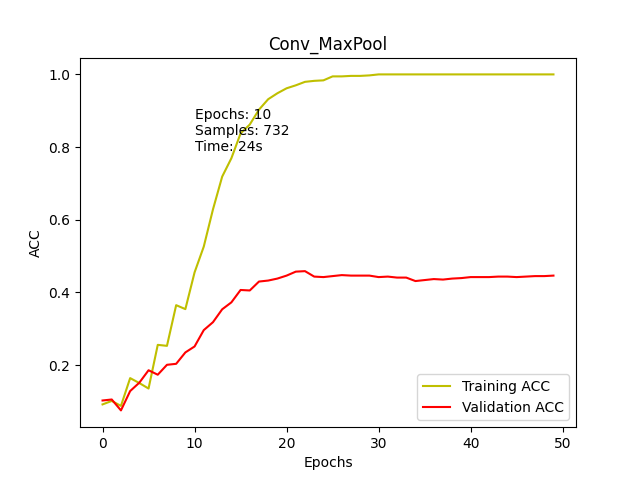
\includegraphics[height=5cm]{../../Plots/ba_plots/convmaxpool/wotr.png}
    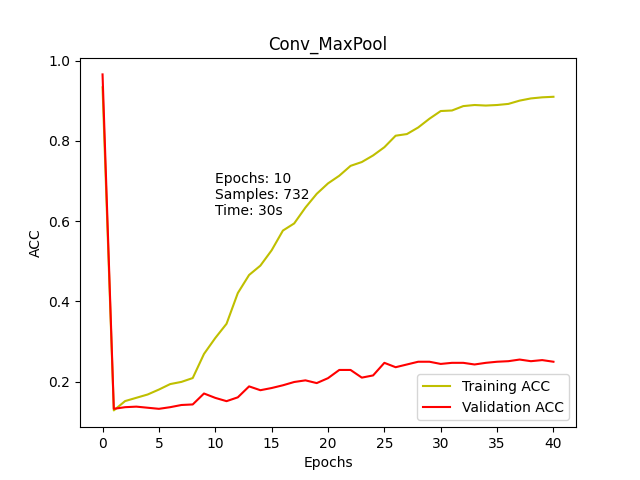
\includegraphics[height=5cm]{../../Plots/ba_plots/convmaxpool/epochTFtr.png}
    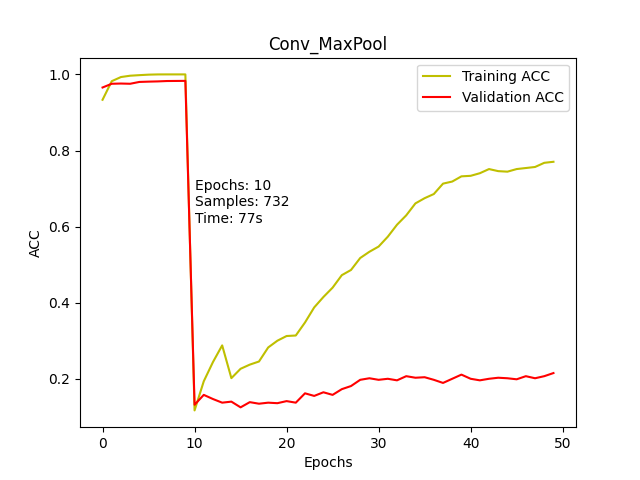
\includegraphics[height=5cm]{../../Plots/ba_plots/convmaxpool/1TFtr.png}
    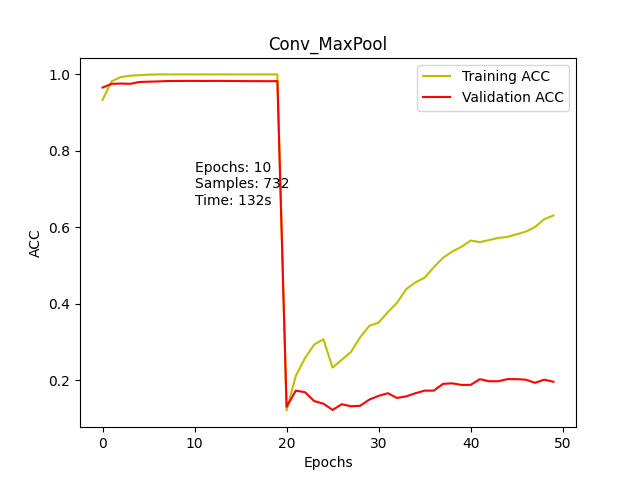
\includegraphics[height=5cm]{../../Plots/ba_plots/convmaxpool/2TFtr.png}
    % 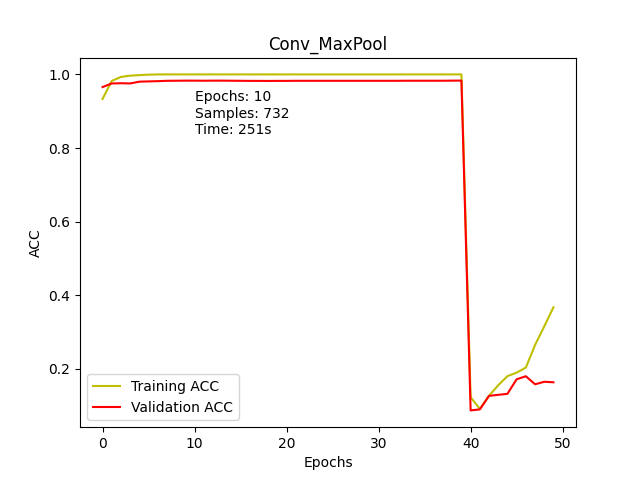
\includegraphics[height=5cm]{../../Plots/ba_plots/convmaxpool/4TFtr.png}
    \caption{\label{fig:layertf} 
    \small{Hier sind von links oben nach rechts unten die Plots folgender Tests zu sehen: 
    CMP:732/10, CMP:TF0/732/10, CMP:TF1/732/10, CMP:TF2/732/10. Alle Plots haben hier dasselbe Problem damit, dass der Unterschied 
    zwischen der Trainings-Accuracy und der Validation-Accuracy immer größer wird.}}
\end{figure}

Auffällig ist es, dass hier die beste Performanz ohne TF ist. Bereits nach nur einer Epoche im ersten Layer, welches auf dem Sourcedatensatz 
trainiert wird, bricht die Accuracy ein. Dies zeigt, dass TF bei Klassifikation und Deep Cascade Netzwerken sinnfrei ist. Das 
Trainingsset der Trainingsdaten kommt bei TF nie auch nur annähernd an den Bereich heran, in dem es ohne TF ist. Daraus folgt, dass es 
bereits zu Overfitting auf dem Sourcedatensatz gekommen ist. Dadurch kann nicht mehr so gut auf dem Targetdatensatz gelernt werden. Dieses 
Overfitting passiert sogar bereits, wenn nur eine Epoche auf dem Sourcedatensatz gelernt wird, was die Graphik oben rechts von Figure \ref{fig:layertf} zeigt. 
Ebenso ist es offensichtlich, dass es bei jedem Graph zu Overfitting auf dem Trainingsset des Targetdatensatzes kam, da dieser um 60\% höhere 
Accuracy als das Validationset und dem Testdatenset vorweist. 

Bei einem Regressionsnetzwerk, wie dem Deep Cascade Netzwerk RegressionTwo kommt es, wie in Figure \ref{fig:regr2tf} zu sehen, nicht so schnell zu Overfitting. 
Es kommt dazu weder auf dem Sourcedatensatz noch auf dem Targetdatensatz. 

\begin{figure}[htpb]
    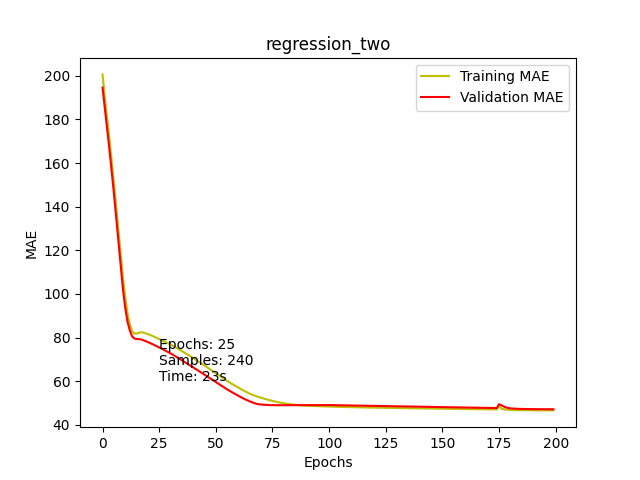
\includegraphics[height=5cm]{../../Plots/ba_plots/regr2/woregr2tr.png}
    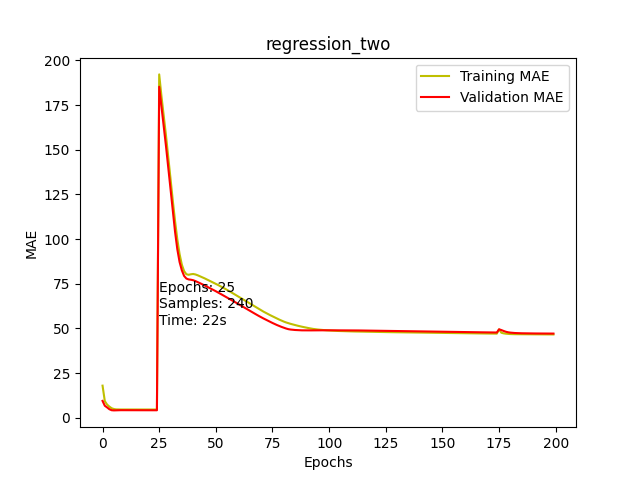
\includegraphics[height=5cm]{../../Plots/ba_plots/regr2/1TFtr.png}
    \caption{\label{fig:regr2tf} 
    \small{Hier ist links der Test Regr2:240/25 und rechts Regr2:TF1/240/25 zu sehen. Der MAE zwischen Trainingsset und Validationset hat kaum 
    einen Unterschied. Hier ist kein Overfitting.}}
\end{figure}

Dieses Overfitting-Problem hat nur die Klassifikation. Dies muss an der Loss-Function oder der Activation-Function, die für Klassifikation 
benutzt wird, liegen. 

\iffalse
Also am CategoricalCrossEntropy oder am Linear. Hinter dem CategoricalCrossEntropy ist folgende Formel: 

\begin{equation}
    CCE = -\frac{1}{M} \sum_{k=1}^{K}\sum_{m=1}^{M} y_m^k * \log(h_w(x_m, k))
\end{equation} 

Dabei ist M die Anzahl der Datensamples, K die Anzahl der Klassen, $y_m^k$ das Target label, x der Input und $h_w$ die 
Gewichte \cite{rwcrossentropy}. 
\fi
